\documentclass{article}
\usepackage{cancel}
\usepackage[utf8]{inputenc}
\usepackage {titlesec}
\usepackage[english,russian]{babel}
\usepackage{amssymb}
\usepackage{amsmath}
\usepackage{graphicx}
\graphicspath{{pictures/}}

\titlespacing*{\section}{\parindent}{*4}{*4}

\title{Домашнее задание 10}
\author{Ткачев Андрей, группа 166}
\date{\today}

\begin{document}
	\maketitle
	\section {Задача 1}
	\subsection{(а)}
	
	Построим граф частичного порядка $P$:
	
	\begin{center}
		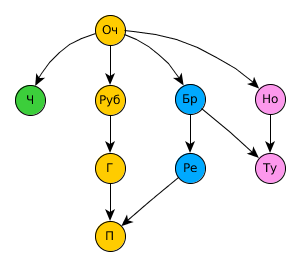
\includegraphics[scale=0.5]{1_1}
	\end{center}
	
	Тогда отношение линейного порядка получается из $P$ таким расположением вершин в линию, что ни из какой вершины нет дуги вверх (т.е. граф ациклический). Пример такого линейного порядка:
	
	\begin{center}
		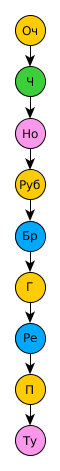
\includegraphics[scale=0.5]{1_2}
	\end{center}
	
	(На иллюстрации, во избежание перегруженности, опустим дуги, которые обеспечивают транзитивность. Здесь и далее будем подразумевать наличие дуг от выше стоящих ко всем ниже стоящим вершинам)
	
	\subsection{(б)}
	
	Количество линейных порядков, содержащих данный частичный  $P$ можно посчитать, узнав число способов соединить <<ветви>> графа порядка $P$ (разные цвета на иллюстрации) в линию, так, чтобы в ней относительный порядок элементов из одной ветви был сохранен.
	
	Поймем тогда, что в любом линейном порядке содержащем $P$, элемент <<Очки>> - максимальный, а <<Часы>> могут располагаться в линии как угодно, но ниже <<Очков>>. Т.е. если мы посчитаем число способов $x$ упорядочить все предметы, кроме часов, то число способов упорядочить те же предметы, но уже c часами - $8x$. Тогда забудем до поры про часы.
	
	Рассмотрим все возможные относительные расположения синих и оранжевых предметов в линейном порядке содержащем $P$. Их всего ${4 \choose 2} = 6$ - по числу способов расположить между очками и пиджаком 2 упорядоченные пары:
	
	\begin{center}
		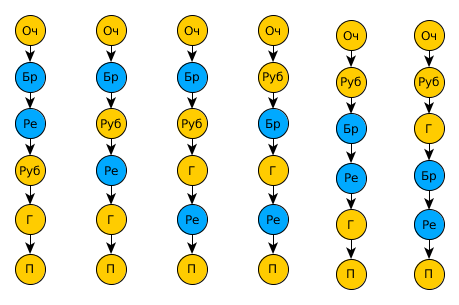
\includegraphics[scale=0.5]{1_3}
	\end{center}

	Для получения линейного порядка в каждое из данных расположений нужно вставить предметы <<Носки>> и <<Туфли>>. Причем <<Туфли>> идут обязательно ниже <<Брюки>>.
	
	Посчитаем количество способов вставит носки и туфли, для каждого из расположений на третьей иллюстрации:
	\begin{itemize}
		\item Первое расположение. Если <<Носки>> идут после брюк, то число способов разместить носки с туфлями, как следует из задачи Муавра (носки и туфли можно воспринимать как перегородки), можно ${4 + 2 \choose 2} = 15$ способами. Если <<Носки>> идут перед брюками (ровно один вариант такого размещения), то число способов разместить носки с туфлями равно числу способов разместить туфли после Брюк, т.е. 5. Всего вариантов $15 + 5 = 20$.
		\item Второе расположение. Аналогично первому, т.к. все зависит только от брюк, которые не меняют своего положения. Всего вариантов $20$.
		\item Третье расположение. Аналогично первым двум: 20 вариантов.
		\item Четвертое и пятое расположение. Рассмотрим случаи, когда носки с туфлями ниже брюк и когда носки выше, а туфли ниже брюк. В первом случае, число способов вставить в порядок носки и туфли по Муавра можно ${3 + 2 \choose 2} = 10$ способами. Во втором случае по правилу произведения разместить носки и туфли можно $2 \cdot 4 = 8$ способами (2 способа надеть носки и 4 - туфли). Всего - 18 вариантов.
		\item Шестое расположение. Разместить носки и туфли ниже брюк можно ${2 + 2 \choose 2} = 6$ способами. Разместить носки, а туфли ниже брюк можно $3 \cdot 3 = 9$ способами. Итого $15$ вариантов.  
	\end{itemize}

	Суммируем и получаем $20 \cdot 3 + 18 \cdot 2 + 15 = 111$ линейных порядков не содержащих элемент <<Часы>>. Добавляем часы в каждый из 93-х порядков одним из 8-ми способов и получаем $111 \cdot 8 = 888$ линейных порядков, содержащих отношение порядка $P$.
	
	\textbf{Ответ: } a) см. иллюстрацию 2;
					 б)888 линейных порядка.
					
	\section {Задача 2}
	Докажем для начала, что ациклическое связное отношение $P$ является отношением строгого частичного порядка. Для этого проверим антирефлексивность, антисимметричность и транзитивность отношения $P$.
	
	\subsection{Антирефлексивность} 
	По условию $P$ - ациклично, т.е. не существует $k$ таких, что если $a_1, \ ...a_k \in A$, то $a_1Pa_2P\ ...Pa_kPa_1$. Значит ни для каких $i$ неверно, что $a_iPa_i$, если $a_i \in A$. Значит $P$ - антирефлексивно.
	
	\subsection{Антисимметричность}
	Если $\exists a_x, \ a_y \in A, \ a_x \ne a_y$: $a_xPa_y$ и $a_yPa_x$, то $P$ не ациклично $\Rightarrow$ таких $a_x, \ a_y$ нет в $A$. Значит $P$ - антисимметрично.
	
	\subsection{Транзитивность}
	Рассмотрим любые попарно неравные $a,\ b,\ c \in A$. Так $P$ - связное отношение, то  $a,\ b,\ c$ как-то попарно соединены, причем по принципу Дирихле есть элемент который входит в отношение $P$ слева и справа. Для определенности, пусть $aPb$ и $bPc$. Но тогда, в силу ацикличности, неверно, что $c P a$. Но тогда в силу связности $a P c$. Значит $\forall a,\ b,\ c \in A\ aPb,\ bPc \Leftrightarrow aPc$. А так как в силу антирефлексивности и антисимметричности $aPb,\ bPc$ возможно только если $a,\ b,\ c$ попарно не равны, то $P$ - транзитивно.
	
	Но тогда $P$ - связное отношение строго частичного порядка $\Rightarrow$ по определению $P$ - строгий линейный порядок.
	
	\section {Задача 3}
	\subsection {(а)} Поможем волшебнику. Пронумеруем города от 1 до $n$. Введем отношение $R$ на множестве городов $A$, и зададим направление движение на дороге между двумя городами $a,\ b \in A$ из $a$ в $b$, если $aRb$. Обозначим за $n(c),\ c \in A$ номер города $c$. Тогда примем $aRb \Leftrightarrow n(a) < n(b)$. Поймем, что в силу того, что номера всех городов различны и мы можем однозначно сравнить номера любых двух городов, $R$ - антирефлексивное, антисимметричное, транзитивное связное отношение, т.е. строгий линейный порядок. Строгий линейный порядок - отношение ациклическое, значит для любого города $c_0 \in A$ не существует $c_1,\ ...c_k \in A$, таких что $c_0Rc_1Rc_2\ ... Rc_kRc_0$. Значит нет такого не пустого маршрута, по которому можно из любого города попасть в него же. Т.е. если выехать из города, то вернуться в него уже нельзя.
	\subsection {(б)}
	Рассмотрим граф дорог между городами. Он представляет собой ацикличный турнир, т.е., как следует из задачи 2, задает отношение строго линейного порядка $R$ на множестве городов $A$.
	Но в любом ацикличном отношении по лемме о существовании максимального(минимального) элемента, существует максимальный(минимальный) элемент $u$, т.е. такой, что $\forall c \ne u \in A:\ uRc\ (cRu) $. Это означает, что существует город, из которого дороги только выходят(в который дороги только входят), а значит в силу того, что любые два города попарно соединены, есть город из которого можно приехать в любой другой и город, из которого нельзя уехать. 
	\subsection {(в)}
	Докажем для начала, что такой путь вообще существует.
	 
	Как мы помним, такая ориентированная система дорог однозначно задает строгий линейный порядок $R$ на множестве $A$. По лемме о существовании максимального элемента, в множестве $A^{\prime}$, на котором задан строгий линейный порядок, найдется элемент $u$,  такой что $\forall a \ne u \in A^{\prime}: u R a$. Тогда из множества городов $A$ возьмем тот самый город, из которого достижимы все остальные по пути длины 1, и исключим его и все дороги из него исходящие из системы коммуникаций Вестероса. Поймем, что оставшиеся дороги и города по-прежнему задают связное ацикличное отношение, т.е. линейный порядок, а значит мы можем повторить только что проделанное но уже с подмножеством $A^{\prime} \subseteq A$. Будем повторять указанные действия по индукции. В силу конечности $A$, мы достигнем ситуации, когда останется один город без дорог, который мы так же удалим. Тогда выпишем все города в порядке удаления из $A$: 
		$$c_1,\ c_2,\ ...c_n$$
	
	Поймем, что $\forall 1 \leq i \leq n:$ есть дорога из $c_i$ в $c_{i + 1}$, т.к. на $i$ операции удаления $c_i$ был максимальным элементом и имел прямую дугу ко всем городам в оставшемся множестве. Т.е. существует путь проходящий по всем городам.
	
	Докажем его единственность. Пусть существует путь $b_1,\ b_2,\ ...b_n$. В силу транзитивности отношения $R$, $b_1$ соединен со всеми городами $b2,\ ...b_n$, но тогда $b_1$ совпадает c $c_1$ (в силу единственности максимального элемента). По индукции $b_i$ совпадает c $c_i$ (т.е. база: $i = 1$; предположение: $b_1,\ ... b_k$ совпадают с $b_1,\ ... b_k$; переход: рассмотрим оставшиеся города $b_{k + 1},\ ...b_n$, в силу предположения это множество совпадет с тем, что было получено после $k$-ого удаления максимального элемента при построении пути, а в силу транзитивности и единственности максимума $b_{k + 1}$ совпадает с $c_{k + 1}$). Т.е. любой путь, проходящий по всем городам совпадает с приведенным.  
	\subsection {(г)} Количество способов ввести отношение строгого линейного порядка на множестве из $n$ элементов равно $n!$ (т.е. $n$ способами выбрать максимум, затем $n - 1$ способом выбрать второй после максимума и т.д.).
	
	\section {Задача 4}
	Поймем, что если $P$ - турнир, то $xPy$ только если $x \ne y$ и $y\bar{P}x$. Тогда рассмотрим три попрано различные альтернативы $a, b, c$. В силу того, то они попарно различны, любые две из трех альтернатив входят в отношение $P$. Тогда возможны всего два не изоморфных варианта попарных отношений $a,\ b,\ c$:
	
	\begin{center}
		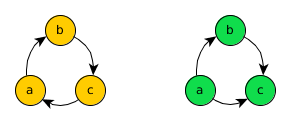
\includegraphics[scale=0.5]{4_1}
	\end{center}

	Тогда, либо существуют три такие альтернативы $a,\ b,\ c$: $aPb \ bPc \ cPa$, либо для любых наборов $a,\ b,\ c$ можно без вреда общности сказать, что $aPb,\ bPc \Leftrightarrow aPc$. А так как $P$ - связно и две альтернативы связаны отношением $P$, только если они различны, то второй вариант означает, что $P$ - транзитивно. Но тогда $P$ - связное отношение строго частичного порядка, т.е. $P$ - строгий линейный порядок.
	
	\section{Задача 5}
	Пусть $P$ - отношение порядка на множестве из $n$ 
	элементов, в котором есть только одна пара несравнимых элементов.
	
	Поймем, что два элемента $x,\ y\ (x \ne y)$ не сравнимы в $P$ тогда и только тогда, когда не существует $z$ такого, что yf   ($xPz$ и $zPy$) или ($yPz$ и $zPx$), иначе, в силу транзитивности $P$: $xPy$ или $yPx$.
	
	Но тогда, если для $z$ верно, что $zPx$, то верно и что $zPy$. Аналогично, если $xPz$, то и $yPz$. То есть в $P$ $x$ не отличим от $y$, т.к. они одинаково соотносятся со всеми прочими элементами. Выберем тогда какие-то 2 элемента из множества, на котором определено $P$, которые будут несравнимы, ${n \choose 2}$ способами. Тогда количество вариантов отношений порядка $P$ в которые не входят фиксированные $x$ и $y$ равно $(n - 1)!$, т.е. числу линейных порядков на множестве из $n - 1$ элемента, т.к. если объединить (в силу одинакового соотношения с прочими элементами) $x$ и $y$ в $x^{\prime}$, то мы получим строгое линейное отношение порядка, которое однозначно соответствует отношению $P$.
	
	Тогда всего отношений порядка на $n$ элементном множестве, в которых ровно два элемента не сравнимы: $(n - 1)! \cdot {n \choose 2}$.
	
	\section{Задача 6}
	Пусть $P$ - некоторый частичный порядок на $n$ элементах. Если $\not \exists\ a, b: (a, b) \notin P \ (b, a) \notin P$, то $P$ - линейный порядок, а значит представимо в виде пересечения не более $n^2$ линейных (при натуральных $n$, $1 \leqslant n^2$).
	
	Пусть тогда $\exists\ a, b: (a, b) \notin P,\ (b, a) \notin P; a \ne b$. Любой частичный порядок представим в виде пересечения линейных его содержащих по теореме Душника — Миллера, следовательно существуют хотя бы два линейных порядка $L_1$ и $L_2$, таких что, $P \subseteq L_1$ и $P \subseteq L_2$, и $ (a, b) \notin L_1\cap L_2,\ (b, a) \notin L_1\cap L_2$, так как иначе любое пересечение линейных порядков содержащих $P$ содержит так же и $(a,\ b)$ или $(b,\ a)$, значит и в $P$ элементы $a$ и $b$ сравнимы, что не так по предположению. 
	
	Тогда для каждой пары $(a, b)$ не сравнимых элементов существует хотя бы два линейных порядка  $L_1$ и $L_2$, таких что $aL_1b$ и $bL_2a$, а $P \in L_1\cap L_2$, т.е. эти элементы не сравнимы в $L_1\cap L_2$. Пусть в $P$ - $k$ пар не сравнимых. Тогда $P$ представимо в виде пересечения не более чем $2k$ линейных порядков - на каждую пару несравнимых берем и пересекаем по два линейных порядка. Всего несравнимых пар элементов может быть ${n \choose 2} = \frac{n(n - 1)}{2}$, значит любой строгий частичный порядок представим в виде пересечения не более чем  $2\cdot {n \choose 2} = n(n - 1)$ линейных. В случае не строгого частичного порядка мы лишь требуем, чтобы $\forall a:\ aPa$ и $aL^{\prime}_ia$ и повторяем рассуждения.

	\section{Задача 7}
	
	\subsection {(а)}
	Если $a\ I_p\ b$, то $(a,\ b) \notin P$ и $(a,\ b) \notin P^{-1}$. Тогда $(a,\ b) \notin P \cup P^{-1}\ \Leftrightarrow\ a\ \overline{P \cup P^{-1}} \ b\ \Leftrightarrow a\ \overline{P} \cap \overline{P^{-1}} \ b\ \Leftrightarrow I_p = \overline{P} \cap \overline{P^{-1}}$.
	
	\subsection {(б)}
	Если $P$ - слабый порядок, докажем, что $I_p$ - отношение эквивалентности, проверив рефлексивность, симметричность и транзитивность.
	
	\begin{itemize}
	\item \textbf{Рефлексивность}
	
	$P$ - строгий частичный порядок $\Rightarrow\forall a\  a\overline{P}a $ и $a\overline{P^{-1}}a$, т.к. $P$ - не рефлексивно. Значит $\forall a\ a \overline{P} \cap \overline{P^{-1}} a \Rightarrow a\ I_p\ a$.  
		
	\item \textbf{Симметричность}
	
	Пусть $I_p^{-1} = (\overline{P} \cap \overline{P^{-1}})^{-1} = (\overline{P}) ^ {-1} \cap (\overline{P^{-1}})^{-1} = \overline{P^{-1}} \cap \overline{P} = \overline{P} \cap \overline{P^{-1}} = I_p$.
	
	\item \textbf{Транзитивность}
	
	Пусть $aI_pb$ и $bI_pc$. Тогда, т.к. $I_p \subseteq \overline{P}$, $a \overline{P} b$ и $b \overline{P} c$. Но $P$ - слабый порядок, значит $a \overline{P} c$. В силу симметричности $bI_pa$ и $cI_pb$. Тогда, $c \overline{P} a\ \Rightarrow$ либо $a = c$ и $aI_pc$, либо $a \ne c$. Во втором случае $(a, c) \notin P$ и $(c, a) \notin P$ $\Rightarrow (a, c) \notin P^{-1}$ $\Rightarrow (a, c) \in \overline{P^{-1}}$, а значит $a \overline{P} \cap \overline{P^{-1}} c \Rightarrow aI_pc$.
\end{itemize}
	Докажем в обратную сторону. Т.е. если $I_p$ - отношение эквивалентности, докажем, что $\overline{P}$ - транзитивно.
	
	Пусть $a\overline{P}b$ и $b\overline{P}c$.
	
	Если $bPa$ и $cPb$, то $cPa \Rightarrow a\overline{P}c$. 
	
	Если $b\overline{P}a$ и $c\overline{P}b$, то $bI_pa$ и $cI_pb$, но тогда $aI_pc$, т.е. $a$ не сравнимо с $c$. Но тогда $a\overline{P}c$.
	
	Если $aI_pb$ и $bP^{-1}c$, то $(a, c) \notin I_p$ - так как иначе по эквивалентности $I_p$: $bI_pc$; значит $a$ сравнимо с $c$. Если $(a, c) \in P$, то по транзитивности $P$-  $aPb$, что не верно, значит $cPa \Rightarrow a\overline{P}c$.  

	Если $aP^{-1}b$ и $bI_pc$, то $(a, c) \notin I_p$ - так как иначе по эквивалентности $I_p$: $aI_pb$; значит $a$ сравнимо с $c$. Если $(a, c) \in P$, то по транзитивности $P$: $bPc$, что не верно, значит $cPa \Rightarrow a\overline{P}c$.

\end{document}